\documentclass{article}


% if you need to pass options to natbib, use, e.g.:
%     \PassOptionsToPackage{numbers, compress}{natbib}
% before loading neurips_2023


% ready for submission
%\usepackage{neurips_2023}


% to compile a preprint version, e.g., for submission to arXiv, add add the
% [preprint] option:
\usepackage[preprint]{neurips_2023}
\usepackage{graphicx}
\usepackage{wrapfig}


% to compile a camera-ready version, add the [final] option, e.g.:
%     \usepackage[final]{neurips_2023}


% to avoid loading the natbib package, add option nonatbib:
%    \usepackage[nonatbib]{neurips_2023}


\usepackage[utf8]{inputenc} % allow utf-8 input
\usepackage[T1]{fontenc}    % use 8-bit T1 fonts
\usepackage{hyperref}       % hyperlinks
\usepackage{url}            % simple URL typesetting
\usepackage{booktabs}       % professional-quality tables
\usepackage{amsfonts}       % blackboard math symbols
\usepackage{nicefrac}       % compact symbols for 1/2, etc.
\usepackage{microtype}      % microtypography
\usepackage{xcolor}         % colors


\title{
  Detecting Sleep States from Accelerometer Data using Deep Learning\\[1ex]
  Alvási fázisok érzékelése gyorsulásmérő adatok alapján mélytanulás használatával
}


% The \author macro works with any number of authors. There are two commands
% used to separate the names and addresses of multiple authors: \And and \AND.
%
% Using \And between authors leaves it to LaTeX to determine where to break the
% lines. Using \AND forces a line break at that point. So, if LaTeX puts 3 of 4
% authors names on the first line, and the last on the second line, try using
% \AND instead of \And before the third author name.

\author{%
  Ádám M. Biró \\
  \texttt{biro.adam@edu.bme.hu} \\
  \And
  Bálint Szalay \\
  \texttt{balint.szalay@edu.bme.hu} \\
  \And
  Zsombor Szenyán \\
  \texttt{zsomborszenyan@edu.bme.hu} \\
  \AND
  \\
  Budapest University of Technology and Economics\\
  Budapest, Hungary \\
}

\begin{document}

\maketitle

\begin{abstract}
  Monitoring sleep patterns is essential when researching sleep and sleep-related problems. Automatically analyzing wrist-worn accelerometer data could emerge as a low-cost and practical method for logging sleep periods when conducting large-scale studies. However, traditional rule-based methods have limited accuracy in detecting sleep onset and wakeup events. In this paper we explore ways how deep learning, a powerful machine learning technique could be used to detect sleep states more precisely. We demonstrate two possible approaches to solve this problem and compare the results.\\[2ex]
  Az alvási minták monitorozása elengedhetetlen fontosságú az alvással kapcsolatos kutatások során. A csuklón hordható gyorsulásmérő adatok automatikus elemzése egy olcsón és egyszerű megoldás lehet az alvási ciklusok rögzítésére nagy mintájú kutatások során. Azonban a hagyományos szabályalapú módszerek nem tudják megfelelő pontossággal meghatározni az elalvás és felébredés időpontját. Ebben a dokumentumban megvizsgálunk lehetséges módszereket arra, hogy a mélytanulást, a gépi tanulás egyik formáját használjuk fel az alvási állapot pontosabb meghatározására. Megmutatunk két lehetséges megközelítést, és összevetjük az eredményeket.
\end{abstract}

\section{Introduction}

Fulfilling sleep plays a crucial role in maintaining physical and mental well–being. Yet a great number of people suffer from problems which negatively affect their sleep patterns. Inadequate quality and quantity of sleep is associated with various health problems, including depression and cardiovascular diseases.

Monitoring sleep patterns is essential when researchers conduct studies on sleep. However, detecting the onset and end of sleep phases is a challenging task. Invasive sleep monitoring methods, such as polysomnography (PSG) are expensive and unsuitable for large–scale studies.

In recent years, wearable devices equipped with accelerometers have emerged as a possible tool for non–invasive sleep monitoring. Traditional techniques which use human–engineered features achieve moderate success in recognizing sleep onset and wakeup events from accelerometer data due to the nuanced transition between sleep and awake states.

A Kaggle competition was hosted by the Child Mind Institute \cite{child-mind-institute-detect-sleep-states} with the goal of finding new approaches to sleep state detection from accelerometer data utilizing the latest advancements in the field of data science.

In this paper we explore the ways how deep learning, a promising machine learning method could be used to solve the task, and also document our models which we created as an entry to the Kaggle competition. Our work also serves as a homework project for the course Deep Learning in Practice at Budapest University of Technology and Economics.\footnote{Deep Learning in Practice with Python and LUA. \url{http://smartlab.tmit.bme.hu/oktatas-deep-learning}}


\section{Dataset}
\label{dataset}

For our model, we used the dataset provided in the Kaggle competition \cite{child-mind-institute-detect-sleep-states}. The training dataset contained about 270 recordings of wrist-worn accelerometer data, annotated with two event types: onset, the beginning of sleep and wake up, the end of a sleep phase. 

The accelerometer recordings are time series data which contain two features: the \textit{z-angle} and \textit{ENMO}. The z-angle is a metric derived from individual accelerometer components that is commonly used in sleep detection, and refers to the angle of the arm relative to the vertical axis of the body. ENMO is the Euclidean Norm Minus One of all accelerometer signals, with negative values rounded to zero. The time series have a resolution of five seconds intervals between data points.

The data was labeled by sleep experts. The following policy was used to label sleep events according to the Kaggle competition description \footnote{\url{https://www.kaggle.com/competitions/child-mind-institute-detect-sleep-states/data}}:

\begin{quote}
"While sleep logbooks remain the gold-standard, when working with accelerometer data we refer to sleep as the longest single period of inactivity while the watch is being worn. For this data, we have guided raters with several concrete instructions:
\begin{itemize}
  \item A single sleep period must be at least 30 minutes in length
    A single sleep period can be interrupted by bouts of activity that do not exceed 30 consecutive minutes
  \item No sleep windows can be detected unless the watch is deemed to be worn for the duration (elaborated upon, below)
The longest sleep window during the night is the only one which is recorded
  \item If no valid sleep window is identifiable, neither an onset nor a wakeup event is recorded for that night.
  \item Sleep events do not need to straddle the day-line, and therefore there is no hard rule defining how many may occur within a given period. However, no more than one window should be assigned per night. For example, it is valid for an individual to have a sleep window from 01h00-06h00 and 19h00-23h30 in the same calendar day, though assigned to consecutive nights
  \item There are roughly as many nights recorded for a series as there are 24-hour periods in that series."
\end{itemize}
\end{quote}

Figure \ref{fig:data-example}. shows an example plot from the input data, a portion of a time series labeled with sleep states.

\begin{figure}
  \label{fig:data-example}
  \centering
  \includegraphics[width=14cm]{fig1.png}
  \caption{A roughly two–day period of a time series data, annotated with sleep states. The upper diagram shows the ENMO signal and the bottom diagram shows the Z–angle signal. The highlighted intervals are labeled as sleep periods.}
\end{figure}

\section{Exploring possible methods}

We began our work by exploring existing work related to the subject. Loh et al. \cite{sleep1} and Malafeev et al. \cite{sleep3} showed that deep neural networks can be utilized for classification of sleep stages based on brainwave signal time series, such as polysomnography (PSG) recordings. Roberts et al. \cite{sleep2} showed that motion sensor data from consumer-grade wearables could possibly be used for sleep stage classification, as there is correlation between motion sensor data and PSG signal data. This led us to believe that deep learning could be successfully used on accelerometer data to detect sleep events. However, the previous works focused on classifying the sleep stage based on an fixed-length window of time series sequences, rather than providing a method to accurately find the boundaries of these stages in an series of arbitrary length.

Typically, the output of a neural network is of a fixed-length. But in our case, the number of sleep onset and wakeup is variable, so we had to design a solution that can produce variable-length output. A straightforward approach would be to divide the time series into smaller segments, as there is at most one sleep period recorded per night. However, this is problematic because there is no hard definition on the boundaries of a night, and the length of a sleep period can vary significantly.

We tried two different approaches to solve this problem: a change point detection based approach and a momentary sleep state classification approach. Below we present the basic principle of these two approaches.

\section{Approach 1: Change point detection (CPD)}

\subsection{Overview}

Change points are points in a time series that mark the boundaries of certain states. In our problem, sleep and awake phases can be viewed as states and the change points represent onset and wake up events. Various methods exist to detect change points using classical machine learning. See Aminikhanghahi et al. \cite{aminikhanghahi17} for a survey of possible methods. Some works have examined the possibility of using deep neural networks for change point detection, notably Li et al. \cite{li2022automatic} and Ebrahimzadeh et al. \cite{multicpd}. We used an approach similar to those that are outlined in these works.

Firstly, we trained a classifier deep neural network to recognize if there is a change point in a given segment of the sensor data series. The input is a fixed-length segment of the sensor data, which we call a \textit{frame}. The output is a one-hot encoded representation of either one of the following three classes: \textit{no event}, \textit{onset}, \textit{wake up}. Then we used a sliding window technique to detect onset and wake up events during the prediction. We employed simple algorithmic methods to merge events that were detected multiple times and filter out sleep periods that are too short or should not be recorded according to the policy described in section \ref{dataset}.

We further refer to this approach as \textit{CPD}.

\subsection{Data preprocessing}
\begin{figure}
    \centering
    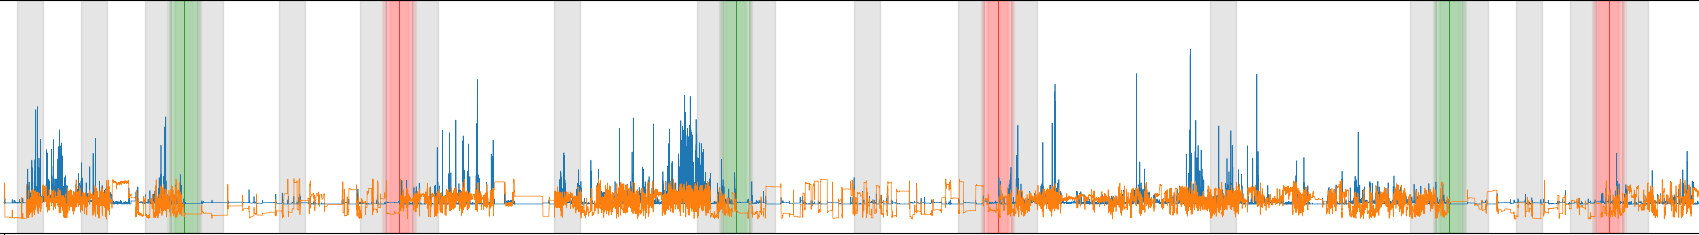
\includegraphics[width=\textwidth]{cpd_sampling.png}
    \caption{A segment of a training sensor series marked with the sampled frames. Grey, green and red frames show sampled frames labeled as \textit{no event}, \textit{onset}, and \textit{wake up}, respectively.}
    \label{fig:cpd-sampling}
\end{figure}

\begin{wrapfigure}{r}{0.33\textwidth}
    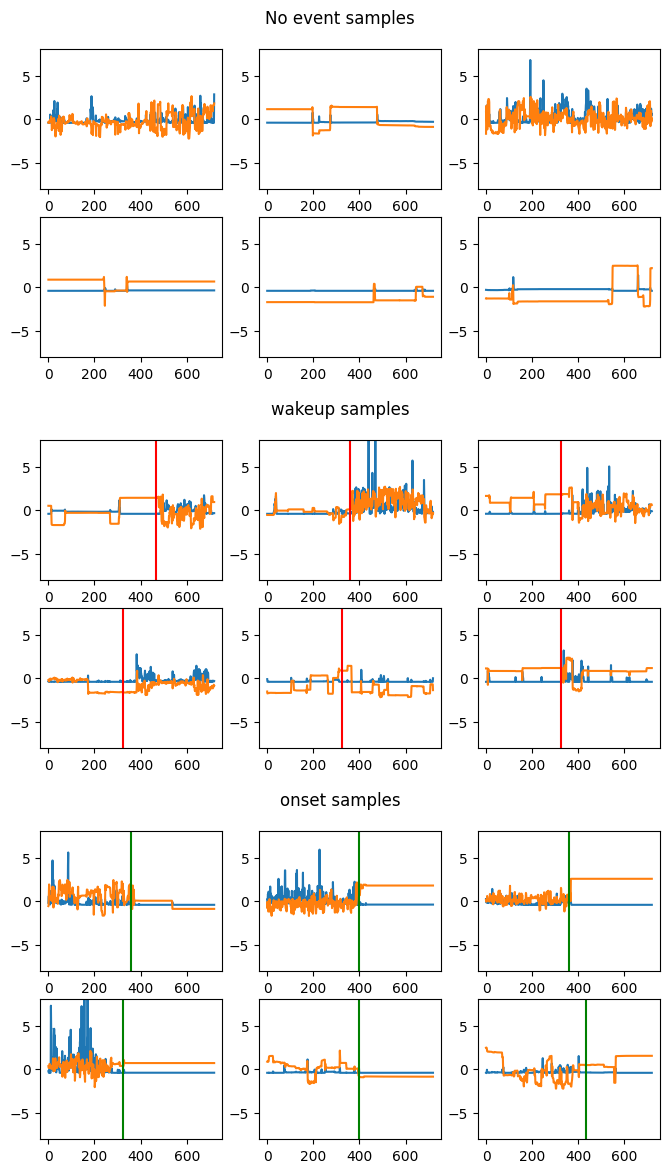
\includegraphics[width=0.3\textwidth]{cpd_samples.png}
    \caption{Training samples in each class extracted from the training data.}
    \label{fig:cpd-samples}
\end{wrapfigure}

We used two features as an input from the time series: ENMO and Z-angle. We standardize the two signals to have zero mean and one standard deviation. Then we sampled frames around ground-truth onset events, wake up events and in between events with the appropriate labels. Figure \ref{fig:cpd-sampling}. shows a segment of a training series marked with sampled and labeled frames. Figure \ref{fig:cpd-samples}. shows example frames that were assigned to each classes. The frame length was set to 60 minutes. Longer frame lengths improved the classification performance, but made the localization of events less accurate as many frames overlapped with one event.

\subsection{Model architecture}

\begin{wrapfigure}{R}{0.33\textwidth}
  \label{fig:model-cpd}
  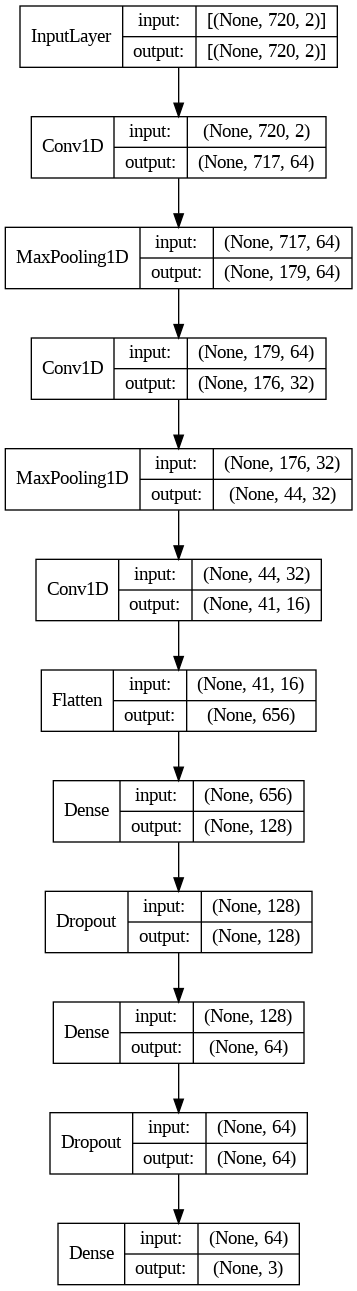
\includegraphics[width=0.3\textwidth]{cpd_model_plot.png}
  \caption{An overview of the neural network of the CPD approach.}
\end{wrapfigure}

We used a multilayered artificial neural network with one-dimensional convolutional layers. Convolutional layers are ideal for extracting features in an input which is indifferent to translation. The model consists of three convolutional layers with additional subsampling layers, and three fully-connected layers. The output layer has softmax activation because the output is an one-hot encoded representation of the predicted class. We used regularization to counter overfitting. The detailed architecture of the model can be seen on figure \ref{fig:model-cpd}.
We also tried a recurrent architecture, but there was no improvement in the classification performance.

\subsection{Training}

For the training we used the Adam optimization algorithm and categorical crossentropy as a loss function. The training dataset contained around 25.000 samples in each class. The best achieved validation loss was 0.18 and with 94\% classification accuracy.

\subsection{Prediction}

We used the following algorithm to make predictions using the trained classifier model:
\begin{enumerate}
    \item Slide a frame-sized window with a stride of 3 minutes. Feed the frame at each window position to the classifier network. If the predicted probability of an onset or wake up event exceeds a certain threshold, record the event accordingly at the center of the window. We got the best results with 0.97 as a threshold.
    \item Combine multiple events of the same type into one event if they are close to each other, which means they probably represent the same ground-truth event. The time step of the new combined event is the average of the combined events.
    \item Determine the sleep periods based on the predicted events with by choosing the longest possible sleep periods. This effectively means sleep periods start when there is a predicted onset before a wakeup event and ends when there is a wakeup event before an onset event.
    \item Merge sleep periods which have a less than 30 minute long gap between them. This is useful because according to the instructions used in recording the ground-truth events, sleep periods can be interrupted with less than 30-minute long bouts of activity (see section \ref{dataset}).
    \item Filter out sleep periods that are shorter than 30 minutes (which are not recorded according to the instructions).
    \item Assign each predicted sleep period to a night based on which \textit{midnight point} it its midpoint is the closest to. Midnight point is a designated time of the day, which we set to 3AM.
    \item Take only the longest sleep period for each night. This is needed because the rest are not recorded according to the instructions. Furthermore this helps to filter out inactive periods during the day which are not sleeping states.
\end{enumerate}

\begin{figure}
    \centering
    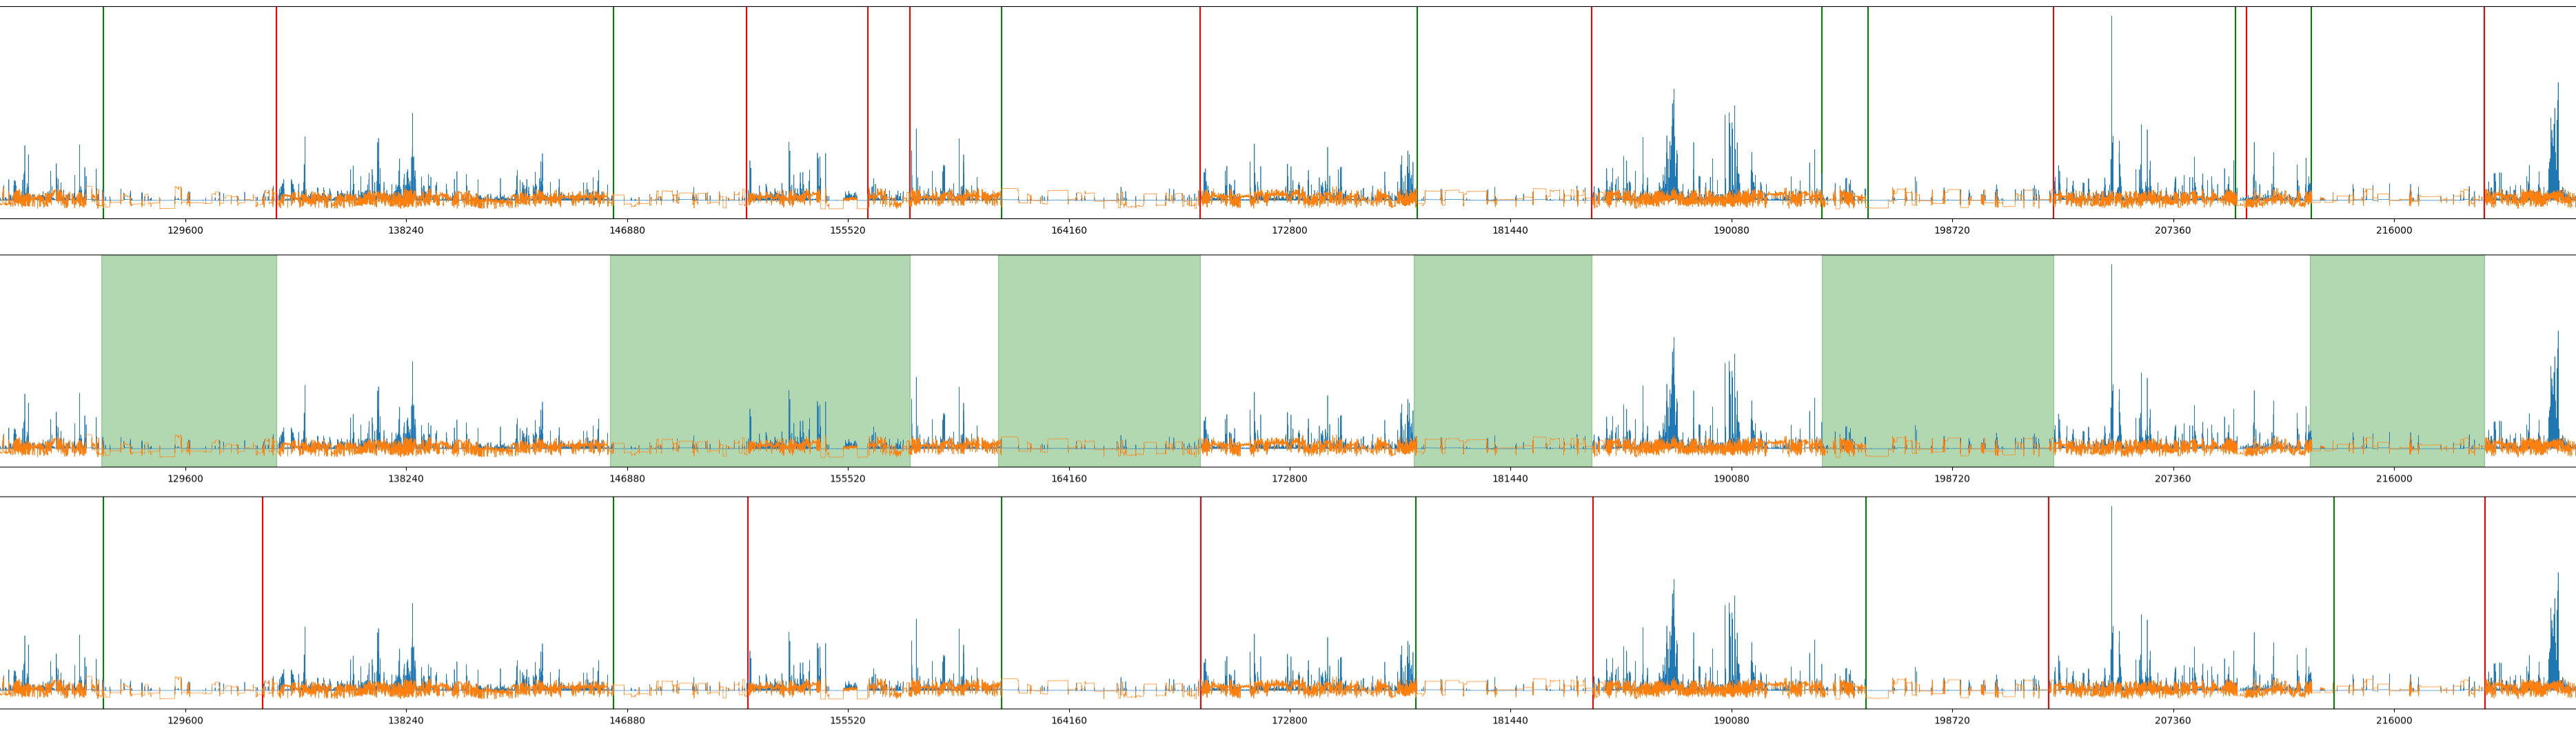
\includegraphics[width=\textwidth]{cpd_prediction_plot.png}
    \caption{An example of result of the prediction algorithm. The uppermost plot shows the combined predicted events, the middle plot shows the fitted and filtered sleep periods. The bottom plot shows the ground truth events. Red lines represent onset events, green lines represent wake up events. The ENMO and Z-angle signals are colored orange and blue, respectively.}
    \label{fig:cpd-prediction-algorithm}
\end{figure}

See figure \ref{fig:cpd-prediction-algorithm}. for a visual example on the algorithm.

\subsection{Overview}

The other method is based on predicting the asleep/awake state in each time step based on a fixed-
length segment of sensor data. In each case, we try to predict whether a person was awake or asleep at each step. There are several attempts for this approach notably Sano et al. \cite{sano19} and Chen et al. \cite{chen21}. We tried to make a classifier based on these approaches.

Firstly, we trained a deep neural network using BiLSTM (see Zargar et al. \cite{zargar21}) to recognize if a person was awake or was asleep at each step in a given segment of the sensor data series. The output represents the probability of a person being awake at each step. Then we used a simple algorithm like the one mentioned in 4.5.

We further refer to this approach as \textit{MSC}.

\subsection{Data preprocessing}
We used one feature as an input from the time series: ENMO. We did not use Z-angle because the model's performance was worse when both ENMO and Z-angle were used. In addition we used two derived features from ENMO. The first was a moving average where we took the average of 7 consecutive values of ENMO. The second was a shifted value, where we took the previous value of the ENMO at the given timestamp. We used min-max scaling for standardization. Then we sampled frames around ground-truth onset events, wake up events and in between events. The frame length was set to 200 timestamp.


\subsection{Model architecture}
We used a multilayered artificial neural network with bidirectional LSTM layers. BiLSTM layers are well-suited for processing sequential data, allowing us to consider context both forward and backward at each step. After that we added a fully-connected layer with sigmoid activation to predict the probability of sleeping. If the probability is closer to 1, then the person was asleep otherwise was awake. We did not use any regularization method, because the model still had difficulty to learn.
The detailed architecture of the model can be seen on figure \ref{fig:model-lstm}.

\begin{wrapfigure}{R}{0.33\textwidth}
    \label{fig:model-lstm}
    \centering
    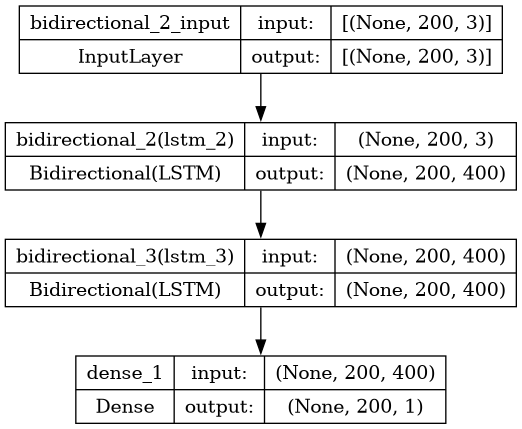
\includegraphics[width=0.3\textwidth]{model_plot-2.png}
    \caption{An overview of the neural network of the momentary classification approach.}
\end{wrapfigure}

\subsection{Training}
For the training we used the Adam optimization algorithm and binary crossentropy as a loss function. The training dataset contained around 4.000 samples in each class. The best achieved validation loss was 0.15.

\subsection{Prediction}
We used the following algorithm to make predictions using the trained classifier model:
\begin{enumerate}
    \item First of all, we had predicted values for each steps. In order to filter out possible anomalies, we took a 240-step long moving average for the probabilities.
    \item After that if the probabilities is higher than 0.5 then at that step the person was asleep so the value of sleeping was 1. Otherwise the people was awake so the value of sleeping was 0. We extracted onset and wakeup events from these values.
    \item[3-6.] Same as in the CPD approach.
\end{enumerate}

\section{Evaluation}

\subsection{Metric}
For the evaluation of the two models, we used a metric called Event Detection Average Precision. This metric is used by Kaggle to score the submissions to the competition. The metric is described on Kaggle as the following:\footnote{Source: Event Detection AP | Kaggle. \url{https://kaggle.com/code/metric/event-detection-ap}}
\begin{quote}
    This metric is similar to IOU-threshold average precision metrics commonly
    used in object detection. For events occuring in time series, we replace the
    IOU threshold with a time tolerance.

    Submissions are evaluated on the average precision of detected events,
    averaged over timestamp error tolerance thresholds, averaged over event
    classes.

    Detections are matched to ground-truth events within error tolerances, with
    ambiguities resolved in order of decreasing confidence.
\end{quote}

We first evaluated the models on 30 randomly series from the original Kaggle training dataset which were not used during the training. Then we submitted the models to the Kaggle competition, which were scored with a private testing dataset. The threshold values used are 1, 3, 5, 7.5, 10, 12.5, 15, 20, 25, 30 minutes as specified by Kaggle.

\subsection{Results}
The two approaches achieved the following scores in the Kaggle competition:

CPD model best score: \textbf{0.367}\\
MSC model best score: \textbf{0.317}

\section{Observations}

Both models performed similarly on the testing data. They were moderately successful in recognizing sleep patterns and scored significantly lower scores than the state-of-the-art solutions. (The competition winner submission scored 0.852.)

The CPD based model is capable of succesfully recognizing almost all ground-truth onset and wake up events, and achieves moderate precision in the localization of the events, which significantly detoriates if the frame size is increased. The greatest limiting factor of the model is that it produces many false-positive predictions, which alter the boundaries of the corresponded sleep periods. It is prone to detecting false positive events partly due to the fact that it only sees a short context of a change point. As a result, this model labels all periods with little variation in sensor data as sleep periods, including intervals where the accelerometer was removed or the subject was resting but was not asleep, which can easily be distinguished from sleep periods when the whole interval is seen.

\bibliographystyle{plain}
\bibliography{sample}

%%%%%%%%%%%%%%%%%%%%%%%%%%%%%%%%%%%%%%%%%%%%%%%%%%%%%%%%%%%%


\end{document}